W procesie tworzenia gry FPS na silniku Unity kluczowym elementem jest skuteczne debugowanie, czyli identyfikowanie, analizowanie i rozwiązywanie błędów w kodzie i mechanice gry. Poniżej przedstawione zostaną niektóre z najważniejszych narzędzi debugujących, które mogą być wykorzystane w tym kontekście.

\paragraph{Unity Profiler}\hspace{-1em} -- to narzędzie, które pozwala na analizę wydajności gry. Pomaga identyfikować miejsca, gdzie gra zużywa najwięcej zasobów komputera (GPU, CPU i pamięć RAM). Dla naszej gry Profiler jest niezastąpiony przy optymalizacji wydajności renderowania i skryptów odpowiedzialnych za obsługę mechanik.

\begin{figure}[h]
        \centering
        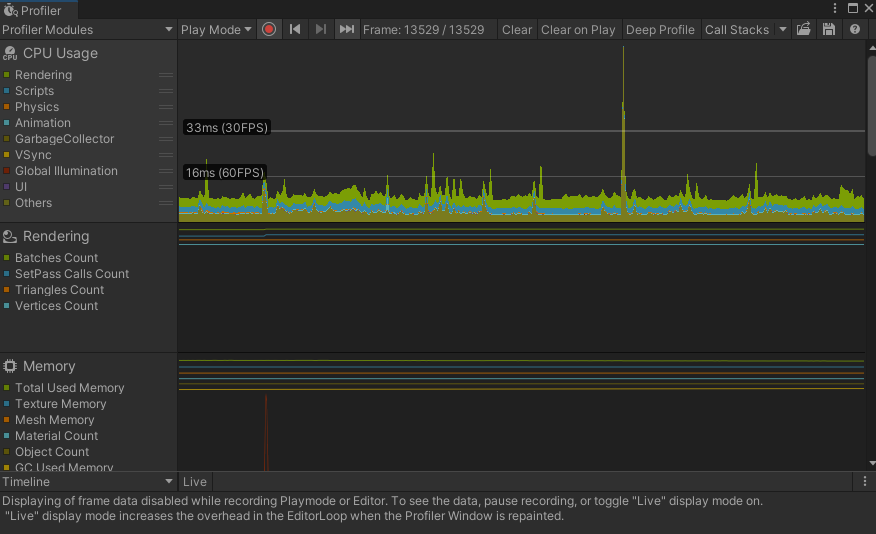
\includegraphics[width=0.9\linewidth]{Images/profiler}
        \caption{Okno Profilera dostępnego w edytorze Unity}
\end{figure}
\FloatBarrier
\paragraph{Unity Frame Debugger}\hspace{-1em} -- to narzędzie dostępne w środowisku Unity, które umożliwia programistom analizę renderowania klatki gry. Jest to szczególnie ważne w grach FPS, gdzie płynność i wydajność renderowania mają kluczowe znaczenie dla doświadczenia gracza.

\begin{figure}[h]
        \centering
        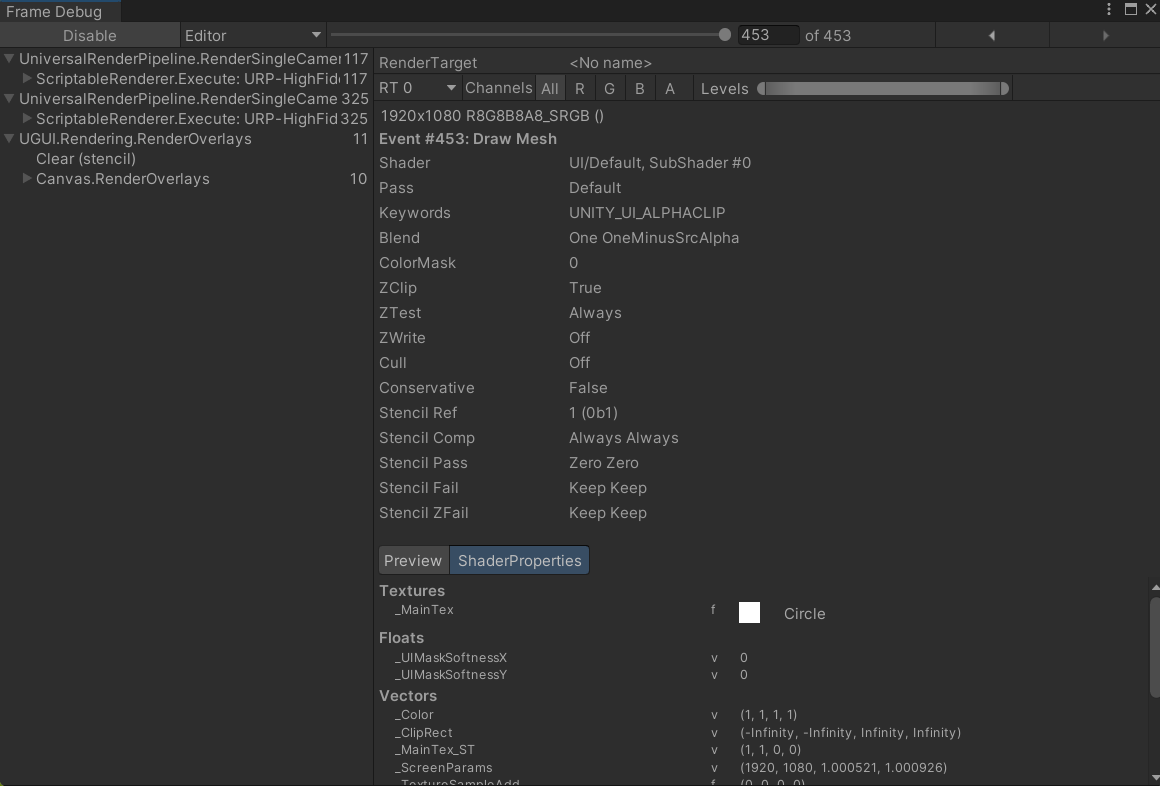
\includegraphics[width=0.9\linewidth]{Images/frameDebug.png}
        \caption{Okno Frame Debuggera w edytorze Unity}
\end{figure}
\FloatBarrier
\paragraph{Unity Console}\hspace{-1em} -- Bardzo prosta ale przydatna konsola dostępna bezpośrednio w edytorze Unity. Wyświetla komunikaty, ostrzeżenia oraz błędy co ułatwia śledzenie zmian i problemów w grze. Konsola bardzo pomaga w identyfikacji problemów związanych z interakcjami z otoczeniem czy działaniem broni.

\begin{figure}[h]
        \centering
        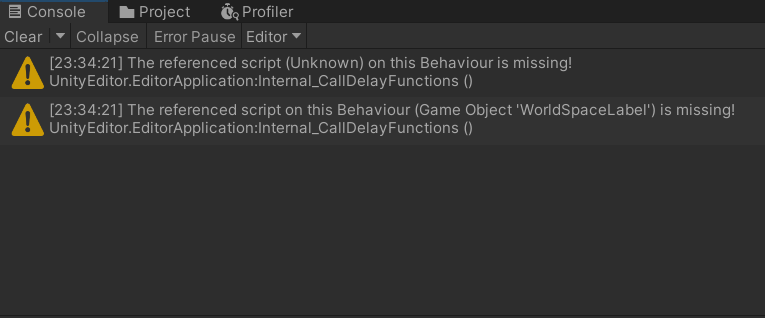
\includegraphics[width=0.9\linewidth]{Images/console.png}
        \caption{Okno Console w edytorze Unity}
\end{figure}
\FloatBarrier